% This file was created with tikzplotlib v0.9.16.
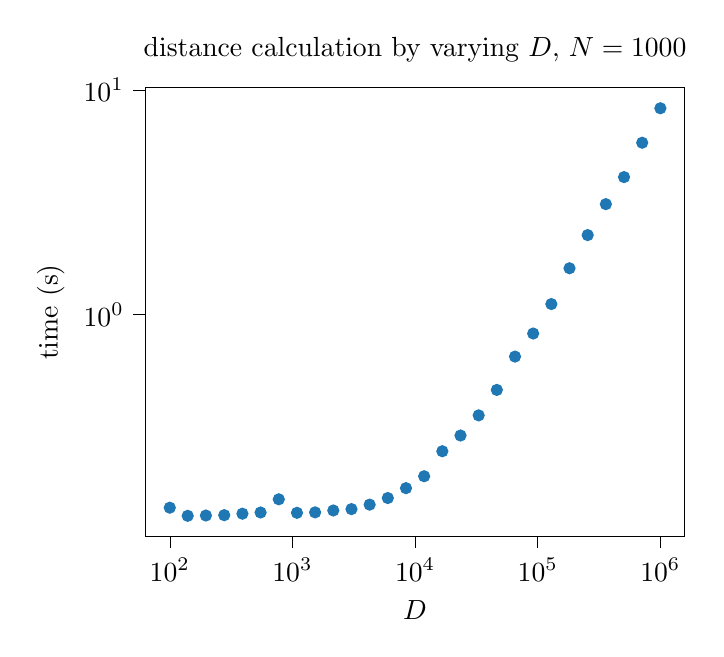
\begin{tikzpicture}

\definecolor{color0}{rgb}{0.12156862745098,0.466666666666667,0.705882352941177}

\begin{axis}[
log basis x={10},
log basis y={10},
tick align=outside,
tick pos=left,
title={distance calculation by varying $D$, $N=1000$},
x grid style={white!69.0196078431373!black},
xlabel={$D$},
xmin=63.0957344480193, xmax=1584893.19246111,
xmode=log,
xtick style={color=black},
xtick={1,10,100,1000,10000,100000,1000000,10000000,100000000},
xticklabels={
  \(\displaystyle {10^{0}}\),
  \(\displaystyle {10^{1}}\),
  \(\displaystyle {10^{2}}\),
  \(\displaystyle {10^{3}}\),
  \(\displaystyle {10^{4}}\),
  \(\displaystyle {10^{5}}\),
  \(\displaystyle {10^{6}}\),
  \(\displaystyle {10^{7}}\),
  \(\displaystyle {10^{8}}\)
},
y grid style={white!69.0196078431373!black},
ylabel={time (s)},
ymin=0.103469157608674, ymax=10.2108433271267,
ymode=log,
ytick style={color=black},
ytick={0.01,0.1,1,10,100,1000},
yticklabels={
  \(\displaystyle {10^{-2}}\),
  \(\displaystyle {10^{-1}}\),
  \(\displaystyle {10^{0}}\),
  \(\displaystyle {10^{1}}\),
  \(\displaystyle {10^{2}}\),
  \(\displaystyle {10^{3}}\)
}
]
\addplot [draw=color0, fill=color0, mark=*, only marks]
table{%
x  y
100 0.138555685679118
140 0.127484877904256
197 0.127895911534627
278 0.128339767456055
391 0.13030997912089
550 0.131924947102865
774 0.151024103164673
1089 0.131466309229533
1531 0.132075230280558
2154 0.134679953257243
3030 0.136567115783691
4262 0.142968575159709
5994 0.152977069218953
8431 0.169279257456462
11859 0.191227515538534
16681 0.247022867202759
23462 0.290161609649658
33000 0.356712023417155
46415 0.462897141774495
65285 0.651361544926961
91825 0.824907143910726
129154 1.11545960108439
181659 1.60957884788513
255509 2.26068615913391
359381 3.10390742619832
505479 4.09477424621582
710970 5.82217709223429
1000000 8.28731513023376
};
\end{axis}

\end{tikzpicture}
